\chapter{Iteracion 2: Primer prototipo de software} % (fold)
\label{cha:iteracion_2}

\section{Introduccion} % (fold)
\label{it2:sec:introduccion}

% fue cuando empezamos a tirar fruta. habiendo elegido el microcontrolador empezamos a probar todas las funcionalidades: El adc, los contadores de eventos, el modulo serial. Despues arrancamos a diseñar el primer prototipo. Consideramos que segun los requerimientos tenia que se un sistema que ofrezca algun tipo de interfaz para que un usuario interactue con el, para que pueda configurarle los parametros segun lo que se quiere lograr.

Los requerimientos de mayor riesgo, son calificados de esta manera porque, de no poder cumplirse, logran que la plataforma sea obsoleta con respecto a sus objetivos principales. La manera de verificar que estos requerimientos son posibles de cumplir, es seleccionar un microcontrolador y luego desarrollar un programa de prueba que compruebe las distintas funcionalidades ligadas a dichos requerimientos. La iteracion anterior fue dedicada a dicha seleccion. En la actual iteracion, verificamos la seleccion mediante un programa basico de prueba.

\subsection{Objetivo de la iteracion} % (fold)
\label{sub:objetivo_de_la_iteracion}

El objetivo principal de esta iteracion, es conformar un primer prototipo de software. Este prototipo no debe necesariamente cumplir con todos los requerimientos, pero si debe verificar el funcionamiento de los modulos del C8051F352 ligados a aquellos requerimientos de mayor riesgo: El conversor analógico-digital; la ganancia programable; los contadores; y el módulo serial.

% subsection objetivo_de_la_iteracion (end)


% section introduccion (end)

\section{Requerimientos de la iteración} % (fold)
\label{it2:sec:requerimientos_de_la_iteracion}

Teniendo en cuenta los requerimientos principiales y el microcontrolador elegido, definimmos los siguientes requerimientos para el software de la plataforma:

\begin{itemize}
\item Se debería poder utilizar el conversor ADC del microcontrolador para transformar señales analogicas de fuentes externas a datos digitales, tanto en modo canal único como canal diferencial.
\item Se debería poder utilizar los contadores del microcontrolador para contar eventos de fuentes externas.
\item Se debería poder utilizar el modulo serial UART y SMBus del microcontrolador para enviar datos a otra placa o microprocesador.
\item Para cada canal del conversor:
\begin{itemize}
\item Se debería poder habilitar y deshabilitar el canal para la medición.
\item Se debería poder configurar el modo de medición (canal único o diferencial). En caso de ser canal único debería especificarse un solo canal, y dos canales para modo diferencial.
\item Se debería poder configurar un tiempo de intervalo entre cada medición.
\end{itemize}
\item Para cada contador:
\begin{itemize}
\item Se debería poder contar eventos con los contadores o timers del microcontrolador.
\end{itemize}
\item Datos de mediciones o meta-datos deberían ser enviados por comunicación serial utilizando protocolo SMBus o UART, según elija el usuario.

\end{itemize}


% section requerimientos_de_la_iteracion (end)

\section{Desarrollo} % (fold)
\label{it2:sec:desarrollo}

En esta seccion se describiran las distintas partes del software y la interaccion entre ellas para cumplir con los requerimientos. Esta descripcion se hara mediante modelos del patron de diseño SysML. El programa en si no fue diseñado mediante este patron, pero realizamos un proceso de ingenieria inversa para facilitar la compresion del lector en el presente informe.

\subsection{Modelos estaticos} % (fold)
\label{it2:sub:modelos_estaticos}

El diagrama de caso de uso de la figura \ref{fig:casouso1}, establece de manera basica aquello que se quiere lograr con el programa embebido en la plataforma. En cada caso de uso, pueden visualizarse las distintas acciones que el programa deberia realizar. Como el programa esta desarrollado en lenguaje C, no es posible conformar un diagrama de clases. En lugar de esto, se separo en distintos modulos que agrupan funciones de caracteristicas similares. Estos modulos estan ilustrados como bloques en la figura \ref{it2:fig:bloquesprimeraiteracionsoftware}. Cada bloque representa distintas partes principales del programa. Se pueden ver los nombres de cada funcion y el tipo de retorno en cada uno de ellos. Con esto ultimo, se intenta dar una idea de las acciones realizadas por las funciones de cada modulo. Una descripcion mas detallada esta en la documentacion del programa \ref{documentacionsoftware}.

El caso de uso ``configurar'' esta generalizado. Las acciones que incluye este caso son:
\begin{itemize}
  \item Configurar la interfaz serial
  \item Configurar canal en modo singular
  \item Configurar canal en modo equilibrado
  \item Configurar contador de eventos
  \item Configurar ganancia del del conversor
  \item Configurar intervalo de medicion para conversion analogica
\end{itemize}


\begin{figure}[h]
  \centering
  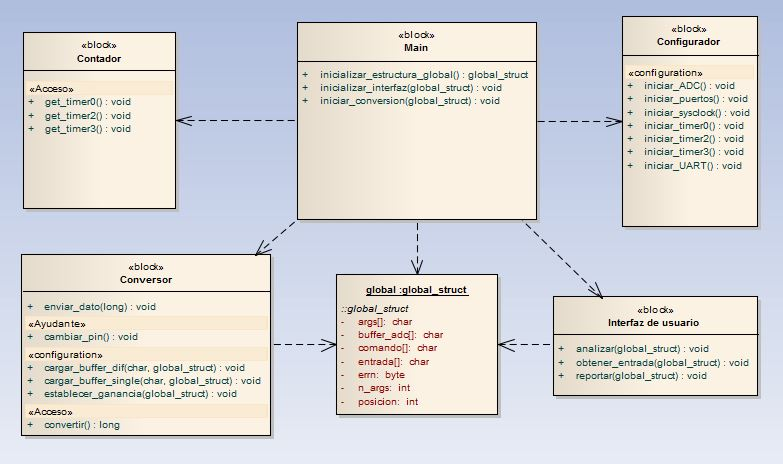
\includegraphics[width=1\textwidth, height = 13.5cm]{bloquesprimeraiteracionsoftware}
  \caption{Diagrama de bloques de la primera iteracion de software}\label{it2:fig:bloquesprimeraiteracionsoftware}
\end{figure}

El objetivo de los diagramas es lograr una descripcion grafica del sistema. Es necesario destacar que, desde el principio, la evolucion del programa ocasiono que los diseños de los modulos fueran cambiando. Los cambios fueron debidos a multiples razones: particularidades del funcionamiento del microcontrolador que no se tuvieron en cuenta, limitaciones del entorno, cambios en los requerimientos, etcetera. 

A continuacion, elaboramos una pequeña descripcion de los bloques que aparecen en el diagrama de la figura \ref{it2:fig:bloquesprimeraiteracionsoftware}.

\begin{itemize}
  \item \textbf{Main o Bloque Principal}: Orquestrador del resto de los modulos. Tiene, ademas, la rutina principal donde se entra al modo de configuracion, para luego iniciar el modo de conversiones continuas.
  \item \textbf{Contador:} Inicializa el hardware de los contadores de eventos del microcontrolador, y contiene las funciones para obtener los valores de los mismos.
  \item \textbf{Interfaz de Usuario:} Levanta la interfaz con la que interactua el usuario para establecer los parametros configurables del sistema, ademas de iniciar el modo de conversiones continuas.
  \item \textbf{Configurador:} Accede a los registros de configuracion de los distintos modulos del microcontrolador. Contiene funciones que realizan todas las configuraciones necesarias para poder hacer funcionar cada modulo del programa.
  \item \textbf{Serial:} Configura el modulo serial para el envio y recepcion de caracteres. Puede ser UART o $I^{2}$C.
\end{itemize}

% subsection modelos_estaticos (end)

Los fabricantes del microcontrolador proporcionan una libreria en C para trabajar con los registros del procesador. Todos los bloques excepto el de la interfaz grafica, manipulan registros para realizar las distintas acciones que le corresponden segun la funcion que se ejecuta.  


\subsection{Modelos dinamicos} % (fold)
\label{it2:sub:modelos_dinamicos}

Utilizamos los modelos dinamicos del patron SysML para describir las distintas interacciones entre los distintos modulos del programa. En esta seccion, describimos las interacciones entre el usuario y el sistema que cubren los requerimientos principales. Las funciones incolucradas en cada interaccion son las mismas declaradas en el diagrama de bloques del sistema. Los distintos flujos que se describen en estos modelos fueron desarrollados iterativamente, es decir, son producto de un desarrollo incremental, hasta llegar al estado que se describe en esta iteracion. \\

Un flujo de ejecucion tipico del programa consiste en una configuracion y un inicio de conversiones continuas. Las conversiones continuas son un loop infinito donde se convierte ciclicamente sobre los canales configurados para la conversion y se envian los datos convertidos por interfaz serial, utilizando el mismo canal serial por donde se realiza el intercambio de comandos para la configuracion. Cuando se interrumpen las conversiones continuas, el programa devuelve al usuario la posibilidad de configurar el sistema, dando fin a las conversiones y el envio de datos. \\

La figura \ref{fig:secuenciaconfiguracionbasica} muestra un diagrama de secuencia para una configuracion de un canal del conversor en modo canal único. Realizada la configuracion, la figura \ref{fig:secuenciaconversioncontinua} muestra como el sistema se establece en modo de conversion continua, entrando en un loop infinito de conversion y envio de telemetria.

\begin{figure}[h]
  \centering
  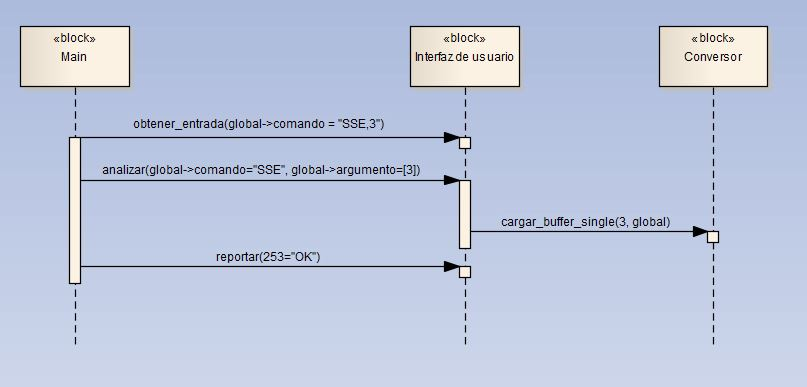
\includegraphics[width=1\textwidth, height = 9cm]{secuenciaconfiguracionbasica}
  \caption{Diagrama de secuencia para una configuracion del conversor. Establece el canal 3 en modo canal unico}\label{fig:secuenciaconfiguracionbasica}
\end{figure}

\begin{figure}[h]
  \centering
  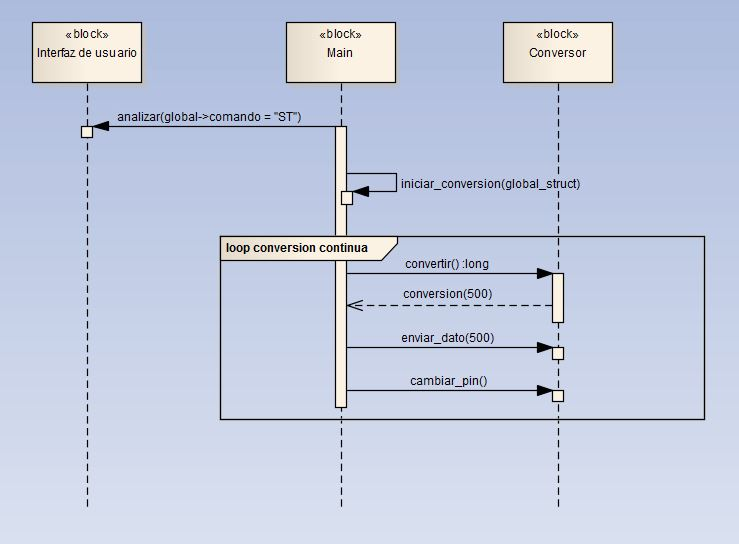
\includegraphics[width=1\textwidth, height = 9cm]{secuenciaconversioncontinua}
  \caption{Diagrama de secuencia para la activacion de conversiones en modo continuo luego de una configuracion previa.}\label{fig:secuenciaconversioncontinua}
\end{figure}



\subsection{El modulo conversor} % (fold)
\label{it2:sub:el_modulo_conversor}

Los registros del microcontrolador permiten manipular el conversor de la siguiente manera (para propositos de la logica de conversion):

\begin{itemize}
  \item Se puede establecer de 1 hasta 8 pines en modo canal unico
  \item Se puede establecer de 1 hasta 4 pares de pines en modo diferencial
  \item Se puede establecer un nivel de ganancia de x2 a x128 para todos los canales
\end{itemize}

Esta lista nos permite concluir que las posibilidades que permite el microcontrolador son limitadas para el uso que se le quiere dar. El modulo conversor del programa deberia, por un lado, permitir la configuracion necesaria de los registros del conversor; y ademas, deberia tener funciones que permitan una configuracion mas compleja de los canales, teniendo en cuenta los requerimientos principales.
Con esto en mente, se desarrollaron distintas funciones que realizan configuraciones segun ciertos parametros de entrada, ingresados por el usuario. Para facilitar la configuracion, se creo un buffer denominado ``buffer de canales''. Este buffer contiene 8 posiciones, y cada una de ellas se corresponde con uno de los canales del conversor. Se elaborara sobre este buffer mas adelante.

Estas son las funciones del modulo conversor:

\begin{itemize}
  \item \textit{convertir}: Interactua con el hardware del microcontrolador para obtener la ultima conversion realizada. Es ejecutada unicamente por la rutina de interrupcion del ADC (iniciada en cada "End of Conversion")
  \item \textit{cargar\_buffer\_single}: Segun un parametro de entrada entero entre 0 y 7, se carga una posicion dentro del buffer de canales con el numero "1", indicando que el canal que se corresponde con esa posicion en el buffer se debe leer en modo canal unico.
  \item \textit{cargar\_buffer\_dif}: Segun un parametro de entrada entero y par entre 0 y 6, se carga una posicion dentro del buffer de canales con el numero "2", indicando que el canal ligado a esa posicion en el buffer, y el siguiente en numero, deben ser leidos en modo diferencial.
  \item \textit{cambiar\_pin}: Cambia el canal por donde se medira en la proxima conversion.
\end{itemize}
% subsection modelos_dinamicos (end)

\subsection{Buffer de canales y logica de cambio de canal en modo de conversiones continuas} % (fold)
\label{it2:sub:buffer_de_canales_y_logica_de_cambio_de_canal_en_modo_de_conversiones_continuas}

Las funciones \textit{cargar\_buffer\_single} y \textit{cargar\_buffer\_dif}, establecen el modo (canal unico o diferencial) en el que se leera un canal. Las 8 posiciones del buffer de canales representan, cada una, un canal distinto del ADC. Los valores posibles para estas posiciones son 0, 1 y 2; estos valores representan, respectivamente, que el canal esta deshabilitado, en modo canal unico, o en modo diferencial. Estas funciones, al ser ejecutadas, cargan algun numero en el buffer según que funcion es la que se ejecuto. El buffer se inicializa por defecto en 0, por lo que inicialmente ningun canal esta habilitado para convertir. \\

Cuando se inicia la conversion continua, se convierte continuamente en un loop infinito. Al final de cada conversion, se llama a la funcion \textit{cambiar\_pin}. Esta funcion utiliza el buffer de canales para obtener cual es el proximo canal a medir. Esto lo hace manejando un indice que comienza en 0, se incrementa hasta 7 y vuelve a 0; recorriendo ciclicamente el buffer de canales. 
En cada ejecucion, analiza una posicion buffer segun el valor del indice. El valor de la posicion del buffer dice si se debe medir en modo canal unico o diferencial, o si es necesario saltear el pin. Una descripcion grafica del comportamiento de esta funcion puede verse en el diagrama de actividades de la figura \ref{fig:actividadescambiarpinit2} \\


\begin{figure}[h]
  \centering
  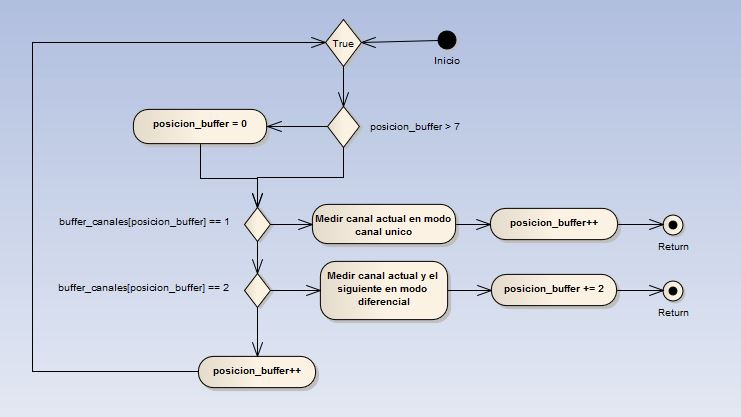
\includegraphics[width=1\textwidth, height = 7cm]{actividadescambiarpinit2}
  \caption{Diagrama de actividad de la funcion cambiar\_pin}\label{fig:actividadescambiarpinit2}
\end{figure}

%Este algoritmo fue el primer prototipo de logica de asignacion y cambio de canal para la lectura de mediciones del conversor. A simple vista es posible ver que los potenciales problemas son muchos. Para empezar, si se asigna el pin 5 en modo canal unico y el modo 4 en modo diferencial, el programa intentara medir en dos modos distintos el mismo canal, dando seguramente resultados inconsistentes. 

% subsection buffer_de_conversion_y_logica_de_cambio_de_canal_en_conversion_continua (end)

% subsection logica_de_las_funciones_del_conversor (end)

\subsection{Logica de las funciones de la interfaz} % (fold)
\label{it2:sub:logica_de_las_funciones_de_la_interfaz}

% Aca es necesario partir el tema en 2.. porque al principio empezamos haciendo todo mal. quisimos hacder una especioe de menu interactivo que le diera la posivilidad al usuario de poder elegir entre distintas opciones de este menu, desplegadas en forma de arbol, para que pudiera elegir la configuracion que quisiera. O sea, arrancaba al principio con un menu general donde ibas navegando hasta poner la configuracion que querias. Asi empezamos, y seguimos con esa logica hasta que se hizo insufrible el programa. Cada vez que queriamos agregar una nueva opcion eran muchas lineas de codigo para cambiar. ahi es cuando investigando me llego el concepto de lo que se llama MMLo "man machine language". Es una logica muy simple. es como un paradigma de interfaz hombre maquina, donde el usuario lo que hace es enviar unos comandos estandarizados y una serie de argumentos, armados en base a una expersion regular. Cisco y Unix Bash usan este paradigma para interactuar con los usuarios. la idea es tan simple como poderosa, lo unico que habia que hacer era decidir como iba a ser el formato de entrada. El analisis posterior es una secuencia que parsea la entrada en busca del comando y los parametros. con el comando, se sabe que funcion ejecutar, y los argumentos son pasados como parametros para esta funcion. Este paradigma es mas complicado de sacar andando, pero es mucho mas escalable que el del menu. a la hora de agregar funcionalidades nuevas se hacia en mucho menos tiempo. Ademas, hace que el programa sea mucho mas facil de testear con unit testing.

La interfaz de usuario tuvo dos implementaciones, siendo la segunda un reemplazo de la primera.

La primera interfaz fue de tipo ``Menu Based Interface'' o interfaz basada en menu, donde las acciones a realizar son ofrecidas por la interfaz y seleccionadas por un usuario. Cada accion esta clasificada segun el grupo de acciones al que pertenezca. Por ejemplo: para configurar el pin 4 del ADC en modo canal unico, es necesario navegar por las opciones del menu de la forma ``configuracion->configurar pin ADC->pin 4->modo canal unico''. Siguiendo este patron de diseño, en cada adicion de una nueva accion, era necesario buscar el grupo al que pertenecia y programar la logica necesaria para ejecutar la accion en base a la navegacion del usuario dentro del menu. Esta forma de desarrollo probo ser muy poco escalable, y fue necesario cambiarla por la dificultad que implicaba a la hora de agregar nuevas funcionalidades. \\

La segunda interfaz diseñada fue de tipo ``Command line interface''. En este tipo de interfaz, el usuario ingresa un comando y uno o varios argumentos en un formato que respeta una expresion regular. Bajo este concepto, se necesita un parser o analizador de comandos que extraiga de la entrada el comando y los argumentos, y realice acciones segun ellos. En nuestro caso, cada comando representa una funcion distinta de nuestro programa, y los argumentos pasan a ser parametros de la funcion. \\

Luego de implementar un analizador de comandos, agregar funcionalidades al programa fue mas simple y rapido con una interfaz basada en linea de comando que con una basada en menu. Por lo que el primer diseño fue descartado y el segundo se mantuvo. \\

\begin{figure}[h]
  \centering
  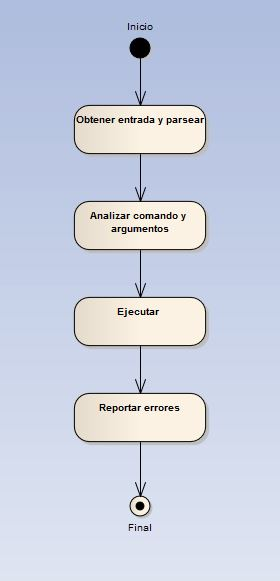
\includegraphics[width=0.40\textwidth, height = 12cm]{actividadinterfaz}
  \caption[Diagrama de actividad del comportamiento de la interfaz de usuario]{Diagrama de actividad del comportamiento de la interfaz de usuario. Se toma la entrada y se parsea para obtener el comando y los argumentos. Segun el comando, se ejecuta una u otra funcion dentro del programa. Los parametros necesarios para ejecutar la funcion se incluyen como argumentos dentro de un arreglo que esta en la estructura global. Este arreglo es luego utilizado por la funcion llamada para obtener los argumentos ingresados junto con el comando.}\label{fig:actividadinterfaz}
\end{figure}

\subsubsection{Formato de los comandos} % (fold)
\label{it2:ssub:formato_de_los_comandos}

Todos los comandos que pueden ingresarse por la interfaz respetan una expresion regular. En el caso nuestro, es la siguiente:

\begin{equation}
\backslash w\backslash w(\backslash w)?(,\backslash d(,\backslash d)?)?
\end{equation}

Dicho de otra manera, el comando ingresado esta conformado por 2 caracteres alfabeticos como minimo y 2 como maximo. El comando puede o no tener argumentos; si los tiene, son dos argumentos como maximo separados por comas, y cada uno es un unico caracter numerico. El comando y los argumentos tambien estan separados por una coma.

% subsubsection formato_de_los_comandos (end)

% subsection logica_de_las_funciones_de_la_interfaz (end)

\subsection{Contadores de eventos} % (fold)
\label{it2:sub:contadores_de_eventos}


El modulo contador contiene las funciones involucradas en el proceso de obtener las cuentas de los contadores de eventos activos en el microcontrolador. Para obtener el valor de una cuenta, simplemente se lee el registro ligado al contador que lleva dicha cuenta. Las funciones de este modulo obtienen la cuenta y la devuelven en forma de cadena de caracteres. \\

Los requerimientos principales indican que es necesario poder contar eventos de 3 o 4 fuentes distintas. Al momento de tomar la decision de cual microcontrolador utilizar, tuvimos en cuenta que este microcontrolador contaba con 4 contadores que podian ser configurados para que tomen fuentes externas para realizar el conteo. En pleno desarrollo del programa, llegamos a la conclusion de que esto no iba a ser posible por las siguientes razones:

\begin{itemize}
  \item El modulo serial del microcontrolador hace uso de uno de los timers para el generador de baudios.
  \item Los timers 2 y 3 comparten la fuente externa de donde ingresan los eventos que se cuentan.
\end{itemize}

Teniendo en cuenta esto, solo es posible contar eventos de 2 fuentes en simultaneo, utilizando timer 0 y timer 2 o timer 3. \\

La reduccion de recursos disponibles para cumplir los requerimientos no fueron suficientes para que sea practico un cambio de microcontrolador, siendo que el resto de las funcionalidades funcionaban correctamente y como era esperado (Con excepcion de SMBus, que se desarrolla mas adelante). Para solucionar este problema, se considero la posibilidad de un diseño de una plataforma con dos microcontroladores, duplicando la cantidad de recursos, y llegando asi al requisito de 4 contadores de eventos de fuentes externas.

% subsection contadores_de_eventos (end)

\subsection{El modulo serial} % (fold)
\label{it2:sub:el_modulo_serial}

Para hacer funcionar el modulo serial, es necesario utilizar uno de los timers como generador de baudios. La implementacion de la funcion que configura el modulo serial del microcontrolador vino ya implementada por Silicon Labs como ejemplo de programa. De todas formas, este ejemplo funcionaba correctamente en nuestro programa y no fue necesario hacerle ningun cambio, mas que modificaciones en el baud rate. \\

Segun los requerimientos, era necesario poder alternar entre SMBus (equivalente a $I^{2}$C) y UART para la interfaz serial. Sin embargo, a pesar de haber realizado multiples pruebas, no fue posible lograr que funcione el modulo SMBus. Luego de acordarlo con el director, decidimos utilizar UART como unico protocolo para la interfaz serial.

% subsection el_modulo_serial (end)

% section desarrollo (end)

\section{Pruebas} % (fold)
\label{it2:sec:pruebas}


\subsection{Tests unitarios} % (fold)
\label{it2:sub:tests_unitarios}

Cada una de las funciones, tanto si interactuan con el hardware del micro como si no, estan testeadas utilizando unit-testing en C, con ayuda del framework ``minunit''\cite{minunit}. Los unit-tests se ejecutaban de la misma manera que se ejecutaba el programa principal, y corria todos los tests, dando como resultado la cantidad de tests que pasaron y los que fallaron.

\begin{table}[h]
\caption{Tests unitarios}
\label{it2:tab:tests_unitarios}
\begin{tabular}{|l|l|
>{\columncolor[HTML]{67FD9A}}l |ll}
\hline
\cellcolor[HTML]{68CBD0}Nombre & \cellcolor[HTML]{68CBD0}Descripcion & \cellcolor[HTML]{68CBD0}Estado &  &  \\ \hline
test\_cargar\_buffer\_unico & intenta configurar un pin enmodo canal unico & {\color[HTML]{009901} Pass} &  &  \\ \cline{1-3}
test\_cargar\_buffer\_diferencial & intenta configurar un pin en modo diferencial & {\color[HTML]{009901} Pass} &  &  \\ \cline{1-3}
test\_GDI & intenta ingresar el comando GDI con combinaciones correctas e incorrectas de parametros, esperando que no haya error en los primeros casos y que si los haya en los segundos & {\color[HTML]{009901} Pass} &  &  \\ \hline
test\_GSE & Analogo a test\_GDI & {\color[HTML]{009901} Pass} &  &  \\ \cline{1-3}
test\_SSE & Analogo a test\_GDI & {\color[HTML]{009901} Pass} &  &  \\ \cline{1-3}
test\_SDI & Analogo a test\_GDI & {\color[HTML]{009901} Pass} &  &  \\ \cline{1-3}
test\_obtener\_entrada & Pide al usuario que ingrese una serie de comandos y verifica que la respuesta del programa sea la esperada & {\color[HTML]{009901} Pass} &  &  \\ \cline{1-3}
test\_iniciales & Compruebael funcionamiento del modulo serial del microcontrolador y el conversor analogico digital & {\color[HTML]{009901} Pass} &  &  \\ \cline{1-3}
test\_blinkled & Prueba el funcionamiento de la plataforma con un programa que hace parpadear un led. Este test esta pensado para ser ejecutado en la plataforma a construir & \cellcolor[HTML]{FF9E9E}{\color[HTML]{CB0000} Fail} &  &  \\ \cline{1-3}
\end{tabular}
\end{table}

% subsection tests_unitarios (end)

\subsection{Tests de sistema} % (fold)
\label{it2:sub:tests_de_sistema}

Las pruebas de sistema se realizaron utilizando la placa de desarrollo mencionada en la seccion PONER ACA LA SECCION DONDE HABLAMOS DE LA SILICON LABS. Al no tener todavia una implementacion hecha del sistema, se utilizo esta placa para testear el codigo embebido en el microcontrolador, que en definitiva seria el mismo que iria en la placa a construir

\begin{table}[h]
\caption{Test de sistema 1}
\label{it2:tab:testsistema1}
\begin{tabular}{p{2cm} p{9cm}}
\multicolumn{2}{c}{\cellcolor[HTML]{68CBD0}{\color[HTML]{000000} Prueba de sistema}} \\
Prueba \#        & 1 \\
\hline
Nombre           & Comportamiento esperado del conversor en modo canal unico   \\
\hline
Requerimiento & Se debería poder recibir datos de sensores analógicos en modo canal unico \\
\hline
Descripcion      & Se conecta un generador de tension en uno de los canales del conversor y se mide en ese canal en modo canal unico, y de esta forma comprobar no tan solo que se este midiendo, sino ademas que estas mediciones esten calibradas para este modo.                                                                                   \\
\hline
Pre-condiciones  & \tabitem Sistema configurado con un pin en modo canal unico \\
                 & \tabitem Generador de tension conectado al pin configurado  \\
                 & \tabitem Computadora conectada al sistema mediante cable serial RS-232 \\
                 & \tabitem Lector de canal serial abierto en la computadora  \\
                 & \tabitem Sistema midiendo en modo de conversiones continuas \\
\hline

Post-condiciones & Los datos de las conversiones que aparezcan en el programa lector de interfaz serial en la computadora deberian corresponderse con los valores de tension provenientes del generador                     
\\
\hline
Secuencia  & \tabitem Establecimos una tension de 1,5 voltios en el generador \\
           & \tabitem La medicion resultante en el lector de canal serial era la misma que la del generador  \\
           & \tabitem Variamos la tension en el generador y la variacion se correspondia en la lectura \\
           & \tabitem Cambiamos a tensiones negativas y verificamos que la lectura daba 0  \\
           & \tabitem Cambiamos a tensiones por sobre la tension de referencia (por defecto 2,5V), y verificamos que el sensor no da valores superiores a 2,5V \\
\hline
Resultados       & Las mediciones dieron resultados coherentes, con algunas variaciones esperadas debido al ruido presente en el ambiente.
\end{tabular}
\end{table}

\begin{table}[h]
\caption{Test de sistema 2}
\label{it2:tab:testsistema2}
\begin{tabular}{p{2cm} p{9cm}}
\multicolumn{2}{c}{\cellcolor[HTML]{68CBD0}{\color[HTML]{000000} Prueba de sistema}} \\
Prueba \#        & 2 \\
\hline
Nombre           & Comportamiento esperado del conversor en modo diferencial \\
\hline
Requerimiento & Se debería poder recibir datos de sensores analógicos en modo diferencial \\
\hline
Descripcion      & Se conecta un generador de tension en uno de los canales del conversor y se mide en ese canal en modo diferencial, y de esta forma comprobar no tan solo que se este midiendo, sino ademas que estas mediciones esten calibradas para este modo. Ademas, se comprueba el funcionamiento de las mediciones en modo diferencial, intentando medir tensiones negativas.                                                                                  \\
\hline
Pre-condiciones  & \tabitem Sistema configurado con un pin en modo diferencial \\
                 & \tabitem Generador de tension conectado al par de pines configurados en modo diferencial. Con el borne positivo en uno y masa en el otro\\
                 & \tabitem Computadora conectada al sistema mediante cable serial RS-232 \\
                 & \tabitem Lector de canal serial abierto en la computadora \\
                 & \tabitem Sistema midiendo en modo de conversiones continuas\\
\hline

Post-condiciones & Los datos de las conversiones que aparezcan en el lector de interfaz serial en la computadora deberian corresponderse con los valores de tension provenientes del generador  
\\ 
\hline
Secuencia  & \tabitem Establecimos una tension de 1 voltio en el generador \\
           & \tabitem La medicion resultante en el lector de canal serial era distinta de la del generador. Leia 2V\\
           & \tabitem Variamos la tension en el generador y la variacion se correspondia en la lectura \\
           & \tabitem Subimos la tension a 1.25V y la lectura dio 2.5V, a partir de ahi, por mas que se subia la tension en el generador la lectura no daba mas de 2.5V. \\
           & \tabitem Cambiamos a tensiones negativas y la lectura no era la esperada pero era consistente. Cuando en el generador habia un 0, leia 1.25V, a medida que la tension se hacia mas negativa, decrementaba aproximadamente al mismo paso que el generador, hasta que el generador llegaba a -1.5V, donde leia un 0  \\
\hline
Resultados       & Las mediciones no dieron los resultados esperados, aunque en si los resultados eran consistentes: los cambios en el generador se reproducian en la medicion, aunque los datos no eran los mismos. Esto se debe a que cuando se mide en modo diferencial, el cero pasa a ser la tension de referencia dividida en dos, para representar los valores negativos. La logica del programa no tenia en cuenta esto, y media las tensiones de forma desfasada.
\end{tabular}
\end{table}

\begin{table}[h]
\centering
\caption{Test de sistema 3}
\label{it2:tab:testsistema3}
\begin{tabular}{p{2cm} p{9cm}}
\multicolumn{2}{c}{\cellcolor[HTML]{68CBD0}{\color[HTML]{000000} Prueba de sistema}} \\
Prueba \#        & 3 \\
\hline
Nombre           & Comportamiento esperado del contador de eventos \\
\hline
Requerimiento & Se debería poder contar eventos con los contadores o timers del microcontrolador. \\
\hline
Descripcion      & Se conecta un generador de onda cuadrada en una entrada GPIO que pueda servir como entrada a algun contador de eventos. Si el contador esta activo, se deberia poder ver que el numero de cuentas incrementa al ritmo de la frecuencia configurada en el generador \\
\hline
Pre-condiciones  & \tabitem Sistema con Timer0 configurado como un contador de eventos activo \\
                 & \tabitem Generador de frecuencia conectado al pin configurado como contador. \\
                 & \tabitem Computadora conectada al sistema mediante cable serial RS-232 \\
                 & \tabitem Lector de canal serial abierto en la computadora \\
                 & \tabitem Lectura continua mediante el canal serial del valor de la cuenta de Timer0\\
\hline

Post-condiciones & El contador deberia contar con una frecuencia igual a la del generador de onda cuadrada
\\ 
\hline
Secuencia  & \tabitem Establecimos una frecuencia de 1000 Hz en el generador \\
           & \tabitem La salida del lector de canal serial mostraba que el contador incrementaba 1000 veces por segundo \\
           & \tabitem Se espero por algunos minutos, verificando que la cuenta sea consistente\\
           & \tabitem Se disminuyo el valor de frecuencia a 100 Hz y se repitio la misma verificacion. \\
           & \tabitem Se disminuyo el valor de frecuencia a 0 Hz y se verifico que el valor de la cuenta quede fijo sin modificarse por 5 minutos\\
\hline
Resultados       & La cuenta era consistente con la frecuencia del generador. El contador de eventos funcionaba correctamente.

\end{tabular}
\end{table}
% subsection tests_de_sistema (end)

% section pruebas (end)
\section{Conclusiones de la iteracion 2} % (fold)
\label{it2:sec:conclusiones_de_la_iteracion_2}

Basandonos en el desarrollo y las pruebas de la iteracion, listamos los avances teniendo en cuenta los requerimientos:

\begin{itemize}
\item El programa utiliza el conversor del microcontrolador para transformar señales analogicas de fuentes externas a datos digitales
\item El programa utiliza los contadores del microcontrolador para contar eventos de fuentes externas
\item El programa utiliza el modulo serial UART del microcontrolador para enviar los datos a otra placa o microprocesador
\item No es posible utilizar el modulo SMBus del microcontrolador.
\item Los datos de conversion correspondientes al numero de pin y el modo de conversion no son enviados junto con la medicion.
\item Para cada canal del conversor:
\begin{itemize}
\item El usuario puede habilitar o inhabilitar el canal para la medicion
\item El usuario puede configurar el modo de medicion (canal unico o diferencial). En caso de ser canal unico especificarse un solo canal, y dos canales para modo diferencial.
\item No es posible configurar un tiempo de intervalo entre cada medicion
\end{itemize}
\item Para cada contador:
\begin{itemize}
\item El usuario puede habilitar o inhabilitar el conteo de eventos.
\end{itemize}
\item No es posible elegir el protocolo serial para comunicarse con la placa o microprocesador externo que recibira los datos, obligadamente debe usarse UART.

\end{itemize}

\subsection{Objetivos para la proxima iteracion} % (fold)
\label{it2:sub:objetivos_para_la_proxima_iteracion}

Teniendo un prototipo de software, lo ideal fue comenzar a pensar en un diseño de hardware en donde hacerlo funcionar. Por lo que el objetivo de la iteracion 3 fue realizar una implementacion de la placa de instrumentacion en un PCB; y una vez construido, realizar las pruebas que aseguren el funcionamiento del mismo.


% subsection objetivos_para_la_proxima_iteracion (end)
% section conclusiones_de_la_iteracion_2 (end)
% chapter iteracion_2 (end)